% preamble
\documentclass[11pt]{article}

% metadata
\title{
  An Implementation of the Quantum Verification of Matrix Products Algorithm
}
\author{Elton Pinto}
\date{}

% packages
\usepackage{amsmath}
\usepackage{amsthm}
\usepackage{amssymb}
\usepackage{braket}
\usepackage[utf8]{inputenc}
\usepackage[margin=1in]{geometry}
\usepackage{parskip}
\usepackage{graphicx}
\usepackage{hyperref}
\usepackage{tikz}
\usepackage{algorithm}
\usepackage{algpseudocode}
\usepackage{caption}
\usepackage{subcaption}
\usepackage{cleveref}
\usetikzlibrary{quantikz}
\usepackage[
  backend=biber, 
  style=ieee,
  url=false,
  doi=false
]{biblatex}
\addbibresource{citations.bib}

\crefname{section}{§}{§§}

% environments
\theoremstyle{definition}
\newtheorem{theorem}{Theorem}[section]
\newtheorem{corollary}{Corollary}[theorem]
\newtheorem{lemma}[theorem]{Lemma}
\newtheorem{definition}{Definition}[section]

\theoremstyle{remark}
\newtheorem*{remark}{Remark}

\newenvironment{solution}
  {\begin{proof}[Sol]}
  {\end{proof}}

% config
\setlength{\parskip}{1em}

% Changes
%
% - Re-read the introduction and background sections
%   - Update/remove any irrelevant portions
% - Update thesis statement (end of introduction and background)
% - Update Materials and Methods
%   - Update experimentatl setup
%   - Add proof of Grover oracle implementation
%   - Add QROM section
% - Update results section
%   - Tables
%     - Swap with newer results (comparison between MPS and statevector)
%   - Figures
%     - Get rid of all figures, replace with newer ones
%   - Analysis
%     - Re-write this section
% - Conclusion
%   - Re-write this section

% document
\begin{document}

\maketitle

\section{Introduction}

Quantum computing has experienced a recent surge in popularity given the
advancements in NISQ machines. Quantum algorithms are known to solve problems
like factoring numbers and simulating natural systems more efficiently than a
classical computer. Companies such as IBM, Google, and Rigetti have recently
built quantum computers that allow researchers to run quantum algorithms on
physical hardware. Given these developments, it has become important to survey
the feasibility of using quantum computing to solve large-scale problems.

Several studies have experimentally evaluated quantum algorithms on quantum
hardware. Mandviwalla et al. evaluated a 4-qubit implementation of Grover
search on the IBM-Q quantum processor \cite{mandviwalla_implementing_2018}.
Similarly, Acasiete et al. evaluated quantum random walks on graphs with 8 to
16 vertices \cite{acasiete_implementation_2020}. However, these studies do not
highlight the challenges involved when scaling to larger-sized circuits.

Similarly, extensive work has been carried out on developing quantum
programming frameworks. IBM has created Qiskit, a Python framework that
supports prototyping and executing quantum algorithms on simulators and quantum
hardware. ORNL is currently developing QCOR, a heterogenous classical-quantum
framework that aims to use quantum computers as accelerators akin to GPUs
\cite{mintz_qcor_2020}. However, little work has been done to evaluate the
efficacy of using these frameworks to develop quantum systems.

Our study aims to fill in these gaps by documenting the process of developing an
oracle for the Quantum Verification of Matrix Products (QVMP)
\cite{buhrman_quantum_2005}\cite{ambainis_quantum_2002} algorithm. This can be
tricky to do given the non-deterministic nature of quantum programs and the
shortage of formal verification tooling in this space. We implement this
algorithm in Qiskit and demonstrate its functionality by running it on the Aer
simulator. We report a proof of oracle correctness, circuit metrics (gate count,
qubit count, circuit depth), transpilation times, and simulation times.

\section{Literature Review}


Quantum computing places an emphasis on thinking about how computation is
performed physically. It achieves speedup over classical algorithms by
exploiting physical phenomenon like entanglement to encode and perform
computation. The main promise of the field is that it can offer a non-trivial
speedup over classical computing. The algorithm that is frequently brought
up to demonstrate this promise is Shor’s algorithm. Shor’s
algorithm provides an exponential speedup over classical algorithms for
factoring numbers and is capable of cracking a subset of the widely-used RSA
encryption. It achieves this by using the Quantum Fourier Transform (QFT), the
quantum analogue of a Fourier transform, to perform phase estimation and
order-finding \cite{nielsen_quantum_2000}.

There are other algorithms like superdense coding, quantum key
distribution, and quantum simulation that have potential applications in
scientific simulation, machine learning, and cryptography. However, these
algorithms tend to require a very large number of qubits to be of practical use.
One of the major challenges in developing large-scale multi-qubit systems is
error-correction and noise. Before we reach the holy grail of  fault-tolerant
quantum systems, the field is currently attempting to make use of Noisy
Intermediate Quantum Computers (NISQ) to solve problems of important practical
use.

Grover's algorithm is a quantum search algorithm that provides an $O(\sqrt{N})$
algorithm for searching through unstructured data, which is a quadratic speed-up
over its classical counterpart. It does this by performing multiple Grover
iteration steps which constructively amplify states that correspond to search
results \cite{nielsen_quantum_2000}. A Grover iteration requires a user-defined
oracle to function correctly. The job of the oracle is to report back whether an
input (encoded as a quantum state) satisfies the search criteria. The core of
Grover search is farily straightforward to implement. The main challenge
here is efficiently encoding the oracle (which is typically described as
a classical decision function) as a quantum circuit. In this study, we try to
better understand this challenge by implementing QVMP which uses Grover search
(and therefore an oracle) as a sub-routine.

There are two popular algorithms for QVMP. The first algorithm, proposed by
Ambainis, Buhrman, Høyer, Karpinski, and Kurur, uses amplitude amplification
along with Grover search to look for a sub-matrix that doesn’t satisfy the
product \cite{ambainis_quantum_2002}. This algorithm runs in
$O(n^{\frac{7}{3}})$ time and improves upon the optimal classical bound provided
by Freivalds \cite{freivalds_fast_1979}. The speedup is obtained because the
algorithm makes use of interference to arrive at a result in a smaller number of
iterations. However, metrics do not exist for the number of qubits required to
implement the oracles for the quantum search algorithms used, and the resources
required to carry out operations like multiplying sub-matrices.  Further, little
research has been done on evaluating the algorithm in a heterogenous
classical-quantum setup where quantum computers are used to accelerate certain
parts of the algorithm. There exists a 4-qubit physical implementation of Grover
search on IBM’s quantum processor \cite{mandviwalla_implementing_2018}. This
implementation tests IBM quantum computers on Grover’s algorithm to investigate
the impacts of different circuit and device attributes, and to highlight the
current capabilities of the system.  This study reports that current quantum
computers are able to solve the search problem on very small data sets. This is
similar to what our study intends to do, however, it does not investigate the
practicality of running algorithms that use Grover search and does not comment
on the composability of circuits and how it affects performance and results. The
second algorithm, proposed by Buhrman and Spalek, uses quantum random walks to
speed up the verification process and runs in $O(n^\frac{5}{3})$ time
\cite{buhrman_quantum_2005}.

Quantum random walks are analogous to classical walks, and have a number of
applications in quantum programming tasks. For example, they are used in solving
the element distinctness problem, in which the goal is to find if there exists a
set of M non-distinct elements in a domain of N elements
\cite{ambainis_quantum_2007}. There have been attempts to run quantum random
walks on quantum hardware. Balu et al.  implemented an efficient physical
realization of a quantum random walk using $log_2(N$ )qubits to represent an
$N$-point lattice \cite{balu_physical_2018}.  Experimental evaluation was
carried out on the IBM-Q five-qubit processor. To overcome resource
requirements, they used a continuous time-limit quantum random walk
implementation. Acasiete et al. have implemented discrete-time quantum random
walks on IBM-Q, and were able to run quantum search based algorithms on graphs
with 8 and 16 vertices \cite{acasiete_implementation_2020}. They were able to
obtain results with 50\% fidelity, and claim that the results are more efficient
than equivalent classical algorithms.

There exists research on resource estimate quantification and benchmarking for
some quantum algorithms. Jaques et al. implemented Grover oracles for key
search on AES and LowMC encryption \cite{canteaut_implementing_2020}. They lay
out a formal description of the oracle,  describe a reversible quantum-gate
implementation of the AES encryption-decryption algorithm, and estimate the
number of Clifford, T, and CNOT gates required for running circuits that can
crack AES-128, AES-192, and AES-256. The project uses Q\#, a quantum
programming language developed by Microsoft. The project reduces the circuit
depth of the Grover oracle by using internal parallelization, in which the
Grover search instance is run on disjoint subsets of the input domain.

A number of open-source frameworks exist for conducting quantum computing
research. IBM provides the Qiskit framework which lets researchers quickly
prototype and test algorithms on a simulator, and also run some workloads on a
quantum computer, the biggest one being the IBM-Q 16-qubit processor in
Melbourne. Fingerhuth et al. have compiled comparisons between Qiskit and other
frameworks like Quil, XACC, and ScaffCC \cite{fingerhuth_open_2018}. They
comment on the programming language choice, documentation, license, and general
culture around these communities. However, they do not compare these frameworks
based on their performance and ability to execute on quantum hardware. LaRose
has compared simulator performance and the quantum compiler of Qiskit and
Rigetti \cite{larose_overview_2019}.  However, the study does not report which
algorithm was used during performance evaluation. Instead, it qualifies a
benchmark based on the number of qubits used. ORNL is currently working on
QCOR, which is a heterogenous framework that aims to enable developers to use
quantum computers as accelerators, much like GPUs \cite{mintz_qcor_2020}. QCOR
doesn’t support amplitude amplification, quantum random walks, and basic
circuits for performing arithmetic as of now. Support will need to be added to
facilitate experimentation using the hybrid classical-quantum programming
approach provided by this framework. Salm et al. has worked on a NISQ analyzer
that determines the best quantum computer system to run a given workload based
on the nature of the quantum algorithm \cite{dustdar_nisq_2020}. They believe
that this will improve developer experience by obviating the need to understand
complicated mathematics to determine the best machine for running a particular
quantum programming task. None of the frameworks currently have a working
implementation of quantum verification of matrix products which we can use to
perform benchmarking.

We believe that it is important to have estimates on how big of an input a
concrete implementation of an algorithm can process. We can use such evaluation
reports to gauge the current state of quantum computing and suggest areas which
need more improvement. Further, we can provide valuable feedback to library
authors about features that need to be added to facilitate productive quantum
algorithm research.

\section{Materials and Methods}

This section covers the major components of QVMP, the algorithm itself,
implementation details, and experimental setup.

\subsection{Grover's Algorithm}

Grover’s algorithm is a popular quantum search algorithm. Given an input space
of $N$ elements and an oracle $U_f$, Grover search can find $M$ solution
indices in $O(\sqrt{\frac{N}{M}})$ time. For simplicity, we assume that $N$ is
a power of 2. 

For $M = 1$ Grover search runs in $O(\sqrt{N})$ time, which is a quadratic
speedup over the classical algorithm for searching in an unstructured database
which takes $O(N)$ time. Therefore, Grover search offers a significant speedup.

The algorithm works by repeatedly applying a Grover operator $G$ to the initial
state $H^{\otimes n}\ket{0}^{\otimes n }$:

\begin{equation}
  (H^{\otimes n}(2\ket{0}\bra{0} - I)H^{\otimes n})U_f = (2\ket{\psi}\bra{\psi} - I)U_f
\end{equation}

It consists of the oracle $U_f$ and a phase shift operator
($2\ket{\psi}\bra{\psi} - I$) known as the diffuser. The specific
characteristics of $U_f$ are described in \ref{sec:grover_oracles}.

Each iteration can be geometrically viewed as a rotation of the state vector in
a plane spanned by the uniform superposition of solutions and non-solutions.
After the application of $U_f$, the diffuser rotates the state vector towards
the superposition of solutions. The number of such iterations can be shown to
be  $O(\sqrt{\frac{N}{M}})$. Therefore, in order to use Grover’s algorithm, one
needs to know the exact number of solutions $M$ in the search space.

The Grover operator circuit is summarized in Fig \ref{fig:grover_operator_circuit}.

\begin{figure*}[!ht]
  \centering
  \begin{quantikz}
    \lstick[wires=5]{$n$ qubits} 
      & \qw 
      & \gate[wires=5][2cm]{U_f} 
      & \qw
      & \gate[wires=5]{H^{\otimes n}}
      & \gate[wires=5]{2\ket{0}\bra{0} - I}
      & \gate[wires=5]{H^{\otimes n}}
      & \qw \\
    & \qw & \qw & \qw & \qw & \qw & \qw & \qw \\
    & \qw & \qw & \qw & \qw & \qw & \qw & \qw \\
    & \qw & \qw & \qw & \qw & \qw & \qw & \qw \\
    & \qw & \qw & \qw & \qw & \qw & \qw & \qw \\
  \end{quantikz}
  \caption{Grover operator circuit}
  \label{fig:grover_operator_circuit}
\end{figure*}


\subsubsection{Grover Oracles} \label{sec:grover_oracles}

The oracle $U_f$ used in Grover’s algorithm can be viewed as black box that
knows how to recognize solutions in the search problem. Let us say we are given
a function $f$ which takes an input $x \in N$ and returns 1 if $x$ is a
solution to the search problem, and 0 otherwise. Then, the action of $U_f$ can
be written as:
\begin{equation}
  U_f\ket{x} \mapsto (-1)^{f(x)}\ket{x}
\end{equation}
Note how the oracle only applies a phase shift to solutions of the search
space. 

The above oracle is commonly implemented by encoding $f$ in a quantum circuit
that flips a target qubit $\ket{y}$ for all inputs $x$ that are a solution to the
search problem. We obtain the phase shift by initializing the target qubit to
the $\ket{-}$ state.

\subsection{Amplitude Amplification}

Amplitude amplification is a generalization of the Grover operator $G$. Instead
of wrapping Hadamard gates $H$ around the diffuser, we now use an arbitrary
unitary $U$.
\begin{equation}
  U(2\ket{0}\bra{0} - I)U^{\dagger}O
\end{equation}
The oracle $O$ behaves in the same way as described in \ref{sec:grover_oracles}.
The unitary can be thought of as a quantum subroutine $A$ that performs a
series of quantum operations without making measurements.

\subsection{Quantum Verification of Matrix Products}

Given three square matrices $A$, $B$, and $C$ of size $n$, the verification of
matrix products (VMP) decides if $AB = C$. Freivalds describes a classical
algorithm which can run in $O(n^2)$ time.

In this paper, we implement the recursive Grover search based quantum VMP by
Ambainis et al. \cite{ambainis_quantum_2002}. The algorithm proceeds by first
partitioning $B$ and $C$ into submatrices $B_i$ and $C_i$ of size $n \times
\sqrt{n}$ respectively. It is easy to observe that $AB = C$ iff $AB_i = C_i \
\forall i$. Now, perform amplitude amplification over the following subroutine:
pick a random vector x, classically compute $y = B_ix$ and $z = C_ix$, and
verify the product $Ay = z$. The verification is done using a Grover search
where the search space is the set of row indices and the oracle verifies if the
inner product between the row and the vector matches the output.

The verification oracle takes $O(n)$ time. Therefore, each Grover iteration
runs in $O(n^{\frac{3}{2}})$ time. We need to run $\sqrt{\frac{n}{\sqrt{n}}} =
n^{\frac{1}{4}}$ iterations of amplitude amplification. Therefore, the overall
running time of the algorithm is $O(n^{\frac{7}{4}})$.

The algorithm is summarized in \cref{alg:qvmp_grover}.

\begin{algorithm}
  \caption{Quantum VMP using Grover Search \cite{j_quantum_2020}}
  \label{alg:qvmp_grover}
  \textbf{Input: } $n \times n$ matrices $A, B, C$ \\
  \textbf{Output: } 1 if $AB = C$ and 0 otherwise \\
  \textbf{Procedure: }
  \begin{enumerate}
    \item Partition $B$ and $C$ into sub-matrices of size $n \times \sqrt{n}$
    \item 
      {
        Perform amplitude amplification for $n^{\frac{1}{4}}$ iterations using this subroutine:
        \begin{enumerate}
          \item Pick a random vector $x$ of size $\sqrt{n}$
          \item Classically compute $y = B_ix$ and $z = C_ix$
          \item Using Grover search with $\sqrt{n}$ iterations, find a row of
            index $j$ such that $(Ay \neq z)_j$
        \end{enumerate}
      }
    \item XOR the sub-results
  \end{enumerate}
\end{algorithm}


\subsection{Implementation}

We implement QVMP in Qiskit, a popular open-source quantum computing platform developed by IBM.
Qiskit uses Python as the host language and has a large libary of utilities that allow
developers to compose non-trivial circuits. It ships with a transpiler and
several backends capable of running circuits on simulators and quantum hardware.

We restrict our implementation to only support binary matrices. Remaining
details can be found in \cref{sec:analysis}.

\subsection{Experimental Setup}

The experiments were run on an AMD EPYC 7502 32-Core Processor, 2.5 GHz, 128
CPUs. The source code is available at \url{https://github.com/1ntEgr8/qvmp}.

\section{Results}

% TODO insert results
% [ ] table - Circuit metrics (using MPS simulator)
  % TODO need more row entries
% [ ] table - Circuit metrics (using Statevector simulator)
  % TODO need more row entries
% [x] fig - Circuit depth before/after transpilation (using MPS simulator)
% ../results/figures/circuit_depth_before_after_transpilation-MPS.pdf
% [x] fig - Circuit depth before/after transpilation (using Statevector)
% ../results/figures/circuit_depth_before_after_transpilation-statevector_cpu.pdf
% [x] fig - Circuit depth vs Transpilation/Simulation time (MPS)
% ../results/figures/circuit_depth_v_tran_time_and_sim_time-MPS.pdf
% [x] fig - Circuit depth vs Transpilation/Simulation time (Statevector)
% ../results/figures/circuit_depth_v_tran_time_and_sim_time-statevector_cpu.pdf
% [x] fig - Circuit depth of MPS vs Statevector after transpilation
% ../results/figures/circuit_depth_of_mps_vs_statevector_cpu.pdf
% [ ] fig - Functionality of QVMP circuit
% [ ]   (a) When there are solutions
% [ ]   (b) When there are no solutions
% [x] fig - QROM example
% ../results/figures/qrom_4x4.tex
% TODO check if QROM matrix is correct
% [x] fig - Inner product example
% ../results/figures/inner_product.tex
% [x] fig - QVMP oracle example
% ../results/figures/qvmp_oracle.tex

% TODO note about MPS vs Statevector
% TODO note about what you benchmarked (just the Grover portion, ideal circuit)
We report the gate counts, circuit depth, and number of qubits used when
targeting Aer simulator in Tables \ref{table:marking_oracle_stats} and
\ref{table:circuit_stats}. Further, we report transpilation times in Table
\ref{table:transpilation_stats}. The sub-circuits used in constructing the
QVMP marking oracle are summarized in figures
\ref{fig:indexer_circuit_3x3} and \ref{fig:inner_product_circuit_3x1}.
Figures \ref{fig:indexer_func} and \ref{fig:inner_product_func}
demonstrate the functionality of these auxiliary circuits. We show the
marking oracle circuit for a 4x4 matrix in Fig
\ref{fig:marking_oracle_4x4}.

\section{Analysis} \label{sec:analysis}

This section describes and analyzes our implementation.

% TODO Note about classical function, segway into QROM and Inner Product
The QVMP oracle is a blackbox that checks if $(Ay - z)_i \neq 0$, where $A$,
$y$, $z$, and $i$ are as defined in the Alg \ref{alg:qvmp_grover}. Qiskit does
not offer tools synthesize oracles using of programming constructs like classical arrays
to a quantum circuit. The programmer has to define these operations on a
per-application basis. The QVMP oracle is composed of the following two
sub-circuits: the indexer circuit and the inner product circuit.

% TODO Explain why QROM is needed, what happens if you use an naive approach
\subsection{QROM}

The role of the indexer is to output $A[i]$, where $A$ is an $m \times n$
matrix and $i$ is an integer index. We encode the matrix $A$ using
$size(A)$ qubits, where $size(A)$ is the total number of elements in $A$.
The integer index is encoded using $log_2(m)$ qubits in the binary format.

If we observe the functionality of the indexer closely, we see that
it is isomorphic to a multiplexer. In other words, the indexer
selects a specific row given a selector (which is the index in our
case). We can implement the indexing operation either as an in-place
(Fig \ref{fig:indexer_circuit_3x3}) or out-of-place operation
(\cite{roy_synthesis_2012}). The in-place solution requires more qubits, while
the out-of-place solution increases the circuit depth and is a little more
tricky to integrate with the rest of the oracle. For simplicity, we decided to
go with the in-place version.
      
Fig \ref{fig:indexer_func} shows the indexer circuit in action. When the index
qubits are not in a superposition state, we measure $A[i]$ with $100\%$
probability. On the other hand, if the index bits are in a superposition, we
measure multiple rows of $A$ depending on the superposition. The index
superposition lets us index multiple rows of $A$ at a time, but we can only
observe one of them when measured.

An interesting point to note is that unlike a classical multiplexer which
checks for the selector bits in parallel, the quantum indexer has to check
every index permutation sequentially. This pattern can be seen in the way
the $X$ gates are applied to the index qubits before applying the Tofolli
gate.

% TODO Talk about how this only works for binary matrices (i.e. in field $F_2$)
\subsection{Inner Product Circuit}

The inner product circuit \ref{fig:inner_product_circuit_3x1}, as the name
suggests, computes the inner product between two vectors encoded as qubits. Our
specific implementation only handles binary numbers (where multiplication is
defined as logical AND and addition as logical OR), but can be easily
extended to support other data types.

The AND operation is done using a Toffoli gate.  The OR gate is then
trivially implemented using De-Morgan's law. Both of these operations are
out-of-place.

% TODO encoding of $A$, $y$, $z$
% TODO uncomputation and why it is required
% TODO Proof of oracle correctness
\subsection{QVMP Oracle}
\begin{figure*}
  \centering
  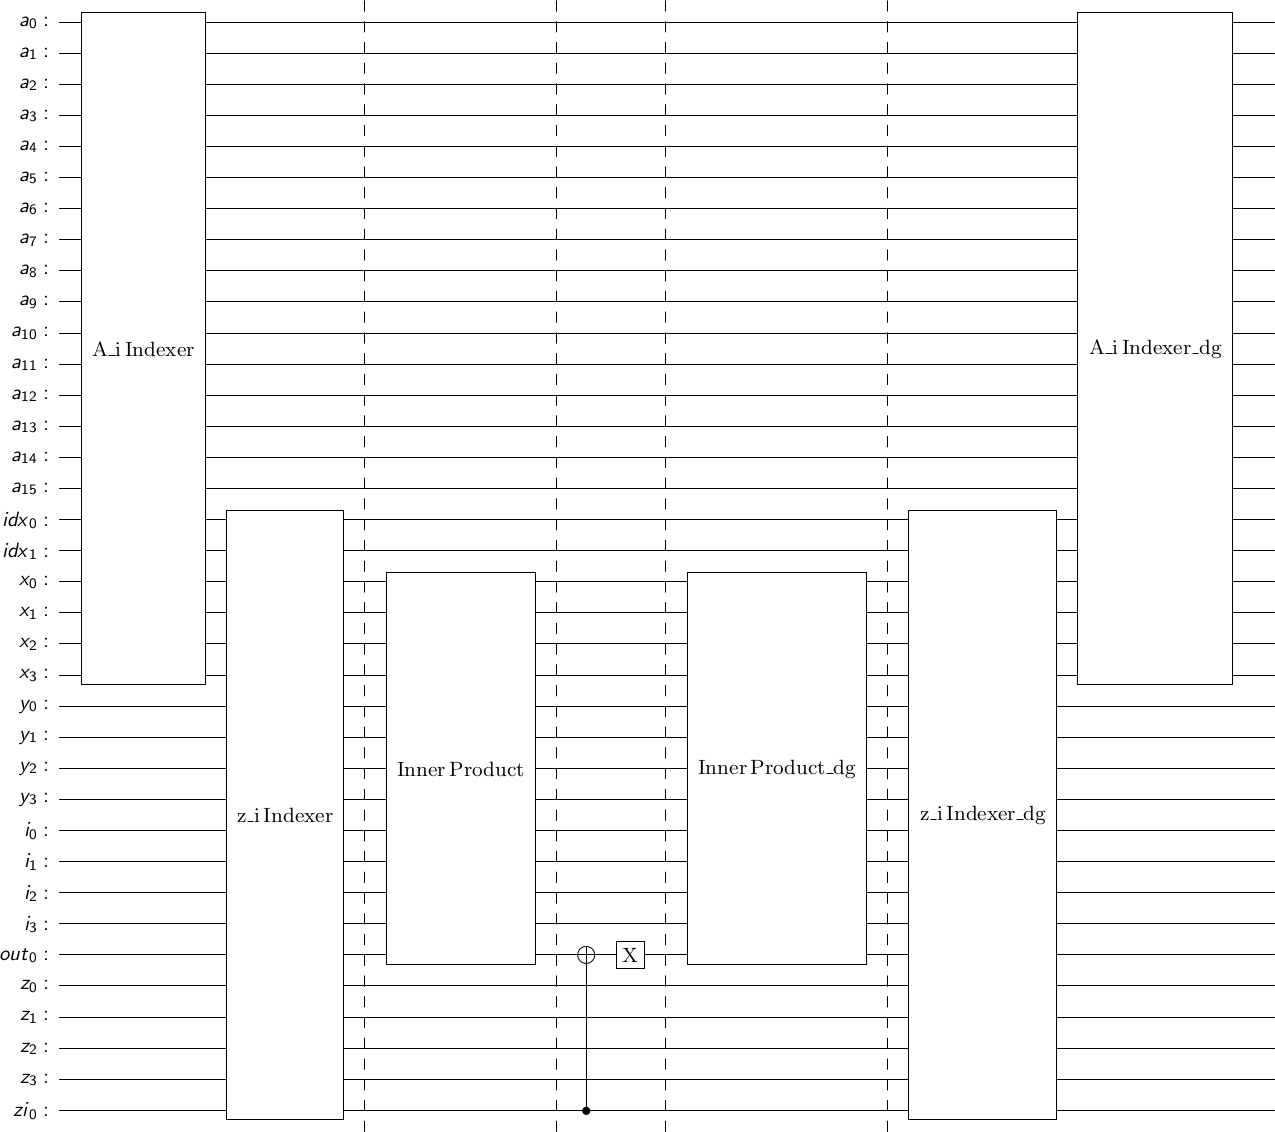
\includegraphics[scale=0.3]{results/oracle_circuit_4x4.png} 
  \caption{QVMP Marking Oracle for a $4 \times 4$ matrix}
  \label{fig:marking_oracle_4x4}
\end{figure*}
The marking oracle (Fig \ref{fig:marking_oracle_4x4}) is composed of both the
indexer and the inner product circuits. We first index into $A$ and $z$
outputting their results into ancilla qubits. Then we compute the inner product
$A_iy$. Finally, we compare the inner product with $z_i$. The comparator
circuit is a CNOT with an additional $X$ gate applied to the target qubit.

As mentioned in Section \ref{sec:grover_oracles}, Grover's algorithm needs an
oracle which performs a phase-flip on correct solutions. We can easily convert
the marking oracle to a phase-flip oracle by simply sandwiching the marker
qubit with $XH$ and its inverse. This has the effect of putting the marker
qubit in the $\ket{-}$ state.

Another important point to note is that the oracle undoes the operations it
carries out in the workspace qubits. This is required so that the next
iteration of Grover can start with a clean workspace. Qiskit simplifies the
process of obtaining the inverse circuits. Every \emph{QuantumCircuit} object has
an inverse method which yields the corresponding circuit.

\subsection{Overall Circuit}

To complete the circuit, we need to apply Grover's search followed by amplitude
amplification. Qiskit provides the \emph{AmplificationProblem} routine which lets
you describe a search problem in the form of an oracle, initial state
preparation, and good states. We use this routine to build the necessary
circuits. For the Grover sub-circuit $G_i$, the state preparation is set to a
Hadamard on the objective qubits. For amplitude amplification, we pass $G_i$ as
the state preparation parameter.

% TODO Note about number of Grover iterations
% When number of solutions are known vs unknown (point back to Results section)

% TODO discussion
% Functionality (for both cases)
  % Number of Grover iterations needed
  % Tradeoff between number of solutions and number of iterations (solving the
  % inverse problem is better)
% Circuit metrics
  % most popular gates, circuit depth (before, after) for MPS vs statevector
    % statevector able to optimize away some gates
  % Qubit count (function of number of columns and rows) (compare to naive case)
  % Number of gates and circuit depth (function of number of grover iterations, number of rows)
% Transpilation vs Simulation times
  % Difference between MPS and Statevector (oppositely shaped charts)

\subsection{Discussion}

Figures \ref{table:marking_oracle_stats} and \ref{table:circuit_stats} show metrics
associated with gate count, qubit count, and circuit depth for the oracle
transpilation and overall circuit transpilation respectively. After
transpilation, the Qiskit compiler decomposes higher-level gates to match the
gate set supported by the backend. We see that the qubit count rises to more
than 4000 for even small matrices of order 32. Further, transpilation onto the
Aer backend added gates that we not part of the high-level design (like $U_2$
and $U_3$). This results in a large increase in the number of quantum
operations performed. The transpilation time rises exponentially with an
increase in the order of the matrix (reaching slightly more than a minute for
an order 24 matrix), thereby slowing the development process.

\subsection{Challenges}

Implementing Grover oracles in Qiskit is cumbersome and error-prone. While the
library offers some routines for automating oracle synthesis, the tooling is
only limited to integers and boolean operators. This makes it challenging to
implement more complex oracles that have succinct classical descriptions.
Grover oracles typically try to emulate a classical operation, and the task of
implementing the oracle amounts to writing the equivalent quantum circuits. We
can develop tooling that takes a classical description of a Grover oracle and
automatically synthesize that into an quantum circuit. Qiskit offers the
classical function decorator to do this, but as mentioned above, it is
only limited to integers. We believe that there is scope to extend the
synthesis to higher-level data types (like arrays and structs) and operators
(like indexing). This will boost developer productivity and make it easier to
iterate on quantum search problems.

Another challenge revolves around verification of correctness. Due to the
non-deterministic nature of quantum computing, it is more nuanced and
challenging to verify outputs. Simulators help alleviate this problem, but they
do not scale very well. For the QVMP case, as highlighted before, compilation
of a circuit for an order 32 square matrix is quite slow. Further, the Aer
simulator can only run circuits using less than 32 qubits. This inhibits the
practicality of algorithms like QVMP. 

As of this writing, NISQ machines support around 50-100 qubits. From Fig
\ref{table:circuit_stats}, this means that we are only able to run QVMP for
matrices of order 4 to 8.  The speedup of the quantum algorithm shows up on
matrices of much larger size.  Quantum noise makes it harder to put QVMP to
practical use. Our findings show that NISQ machines and simulators do not have
the resources to support solving a VMP problem of sufficient size.

\section{Conclusion}

In our study, we implemented the quantum verification of matrix products (QVMP)
algorithm using the Qiskit programming framework. We evaluated our
implementation using gate count, qubit count, circuit depth, and transpilation
time metrics. We detail the mechanics and space complexity of each component of
the circuit and show how they compose together. 

The study reveals that a QVMP circuit of amenable size cannot be run on NISQ
machines due to the number of qubits required to encode the input matrix. It
also highlights the challenges involved in implementing non-trivial quantum
algorithms and how some parts of it (like the synthesis of Grover oracles) can
be automated.

Future work in this space would look to automate the transpilation of a
restricted set of classical functions to quantum circuits using formal
verification techniques if possible. The REVS compiler from Microsoft Research
is a step in the right direction \cite{amy2017verified}. The encoding of
matrices could be improved by using Quantum RAM (QRAM) as outlined in
\cite{giovannetti2008quantum}. This can help reduce the qubit count without
compromising circuit depth.

\newpage

\printbibliography[title=Bibliography]

\end{document}
